\documentclass[conference]{IEEEtran}
\usepackage{cite}
\usepackage{amsmath,amssymb,amsfonts}
\usepackage{algorithmic}
\usepackage{graphicx}
\usepackage{textcomp}
\usepackage{xcolor}
\def\BibTeX{{\rm B\kern-.05em{\sc i\kern-.025em b}\kern-.08em
    T\kern-.1667em\lower.7ex\hbox{E}\kern-.125emX}}
\begin{document}

\title{Trend Correlation on Stack Overflow Programming Languages}

\author{\IEEEauthorblockN{Nicolaus Karamanian}
\IEEEauthorblockA{\textit{University of Victoria} \\
Victoria, Canada \\
nick.karamanian@gmail.com}
\and
\IEEEauthorblockN{Daniel M. German}
\IEEEauthorblockA{\textit{University of Victoria} \\
Victoria, Canada \\
dmg@uvic.ca}
}

\maketitle

\begin{abstract}
Programmers seeking answers to programming related questions have turned Stack Overflow (SO) into the internet's largest programming community. The Q\&A framework of the website has created a forum most programmers ask questions at first. Typically, the number of questions asked for certain programming languages reflects its activity and popularity in the field. We seek to prove this train of thought that posted questions correlate with total usage and popularity in the field. We achieve this by performing correlations on a time series of each language with outside sources: SO annual language popularity surveys, the TIOBE Index, and job postings. We find that in our sample, the SO question amounts correlate strongly with surveys and job postings, but are weakly correlated with the TIOBE Index. To build on this result, we seek to find relations between the programming languages on SO based on the number of questions being asked per language. Certain languages can be found to influence one another in positive or negative ways, such as a language drastically rising in question activity while another language falls, perhaps signifying one language replacing another in the field. We obtain results through time series clustering and linear dependence correlation, and are able to find relations and categorize languages based on the the correlation coefficients.
\end{abstract}

%\begin{IEEEkeywords}
%TODO: do this last.
%\end{IEEEkeywords}

\section{Introduction}
Stack Overflow is the internet's most popular programmer forum. With over 10,000,000 users asking nearly 18,000,000 questions since its inception, Stack Overflow (SO) has become the leading hub for programming specific questions.

On the forum, users post a question relating to a certain programming language's uses, and the other users post answers to said question. The question is labelled with tags relating to the topic in order to categorize said question, the related programming language is usually one of the tags. Users vote on which answers are  helpful or harmful/irrelevant (upvote or downvote), and the original question poster may accept an answer. This framework has led to SO users being able to expect quick and correct answers and also to be unafraid to ask any type of question, whether simple or complex.

SO has grown to the extent that trends among programming languages can be found through the amount of questions being asked. This paper explores the following research questions.

\textbf{RQ1: Does a programming language's activity within Stack Overflow determine its overall popularity?}

\textbf{RQ2: How can programming languages be categorized based on relations found within Stack Overflow statistics?}

\section{Methodology}
To investigate programming language activity on Stack Overflow, we analyze the frequency of questions users post on the forum. We count the number of questions per month users ask pertaining to a certain programming language, and create a time series where each point is a certain month's count. The time series shows the language's activity on SO from August 2008 to current (June 2019). We chose to count by month because a month is long enough to yield a large sample size of questions, yet small enough to view accurate changes in language activity over the 11 year span of data.

Another factor for choosing a month is that we correlate our dataset with the TIOBE Index mentioned below, which is also a monthly dataset. We analyze only languages with a significant user base because languages with very few users produces a very small sample size of questions. The TIOBE Index is a monthly popularity ranking of programming languages based on search engine results. We will consider TIOBE's current top 100 languages as languages with a significant user base.


\subsection{The Dataset}
Stack Overflow releases raw data dumps on Archive.org for public access \cite{datadump}. Of the data dumps they uploaded, we use Posts and Tags data. The Posts xml data contains every post made on SO from August 2008 to June 2019 (at the time of this study), including all questions and answers. Each row of the Posts data contains the content and metadata of a certain post. The Tags xml data contains a list of tags used on SO; each row is a certain tag and its ID number.

We are counting questions per month for certain programming languages, so from Posts we only need the post ID, creation date, post type (question/answer) and the tag IDs (as well as the rating and viewcount for reasons described later). The tags for each post are listed as ID numbers, which we can link to the actual tag (or programming language) in the Tags xml data. We convert the Posts and Tags xml data into csv, and input it into a SQL database for querying. We obtain the monthly question counts for each language by counting the results of queries for all posts created during a certain month with a post type of 1 (question) with a tag ID that represents a certain programming language.

This is our first metric for language activity: question counts per language. The overall rating of each question is the upvote:downvote ratio, so a positive ratio is a question deemed useful by the SO community, and a negative ratio is a question deemed irrelevant or harmful by the community. This adds two more metrics to our data: positively rated and negatively rated question counts per language. Each question also has a viewcount which represents the number of times a question has been visited by other users. Viewcount is another representation of language activity, for example users may be seeking answers to questions already posted.

However, the viewcount for each question is since the question's  creation date and not in monthly format. To normalize the viewcount, we divide the current total viewcount of the question by how many months older it is than June 2019 to give an estimation of its monthly viewcount. This is the fourth and final metric: normalized viewcount per language, henceforward referred to as just viewcount.

\subsection{RQ1: Language Activity and Popularity}

Our current dataset represents the activity of a language within Stack Overflow. To discover if activity within SO represents a language's overall popularity, we look for outside sources to correlate with.

\subsubsection{Stack Overflow Annual Surveys}

Stack Overflow hosts annual surveys \cite{survey} for their users with questions relating to the website as well as programming languages in general. Survey answer data is publicly available. The survey question of interest is what are "The Most Popular Programming, Scripting, and Markup Languages", which was asked in each survey from 2013-2019. We total the answers for each language which yields a ranking of languages each year. From our SO dataset, we total each of the four metrics' monthly counts into yearly totals, which also provides a language's yearly ranking per metric. Maurice George Kendall describes Spearman rank correlation as the most consistent rank correlation method using data with an interval scale \cite{rank}, and Spearman is now the most widely used rank correlation method. Therefore, we calculate Spearman rank correlation to discover if a relation exists between each of our four metrics and the survey answers. Because the users answering the survey come from the same community asking the questions in our dataset, a high correlation will increase the validity of this argument.

\subsubsection{TIOBE Index}

As described above, TIOBE studied search engine results to produce monthly popularity ratings for programming languages, then proceed to rank them for the current month based on their determined rating number \cite{tiobe}. TIOBE does not provide all the past rankings of languages, but they do provide a time series of the ratings for each of the current top 20 languages since June 2001. Figure 1 is an example of said time series for C++. To discover if our SO dataset has a relation with TIOBE's popularity calculation of search engine results, we calculate linear dependence among the set of time series.

To do so, we match by date the monthly count time series of a certain language's four metrics within our SO dataset with the monthly ratings of the TIOBE Index, and calculate a Pearson correlation. A high correlation signifies that the time series trends look highly similar, if not identical.

\begin{figure}[h]
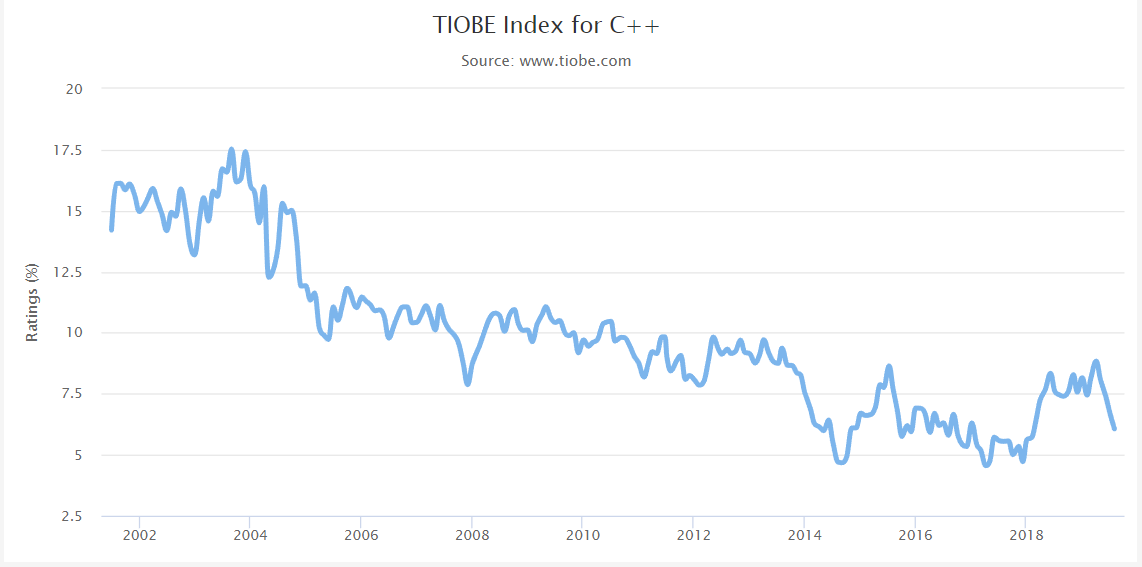
\includegraphics[width=8.5cm]{tiobe_c++.PNG}
\centering
\caption{C++ Ratings on the TIOBE Index}
\end{figure}

\subsubsection{Employability}

Most SO users identify as professional developers, meaning that they use a programming language for employment. We look to discover if one of our four metrics correlates with the employability of a language. To represent a language's employability, we count the number of job postings from employers seeking applicants with skills of a certain programming language. To count job postings, we search for each programming language on large job search websites and count the results. 

For example, for Python we total the counts of the searches "python developer" and "python programming". We do not search just "Python" because some languages such as "C" return many job postings not related to the programming language. We use only two searches, "[language] developer" and "[language] programming", because they consistently return a large set of jobs with mutual exclusion from the other search; other attempted searches produces the same postings found in the aforementioned two searches. 

The number of job postings for each language determine its ranking for June 2019 (the searches done at the time of this paper). We use the monthly counts of each of our four metrics to give each language a rank on SO (a rank for each metric) each month since August 2008. We calculate a Spearman rank correlation for each month in our dataset and the current job postings. A high correlation suggests that the metric used is a good representation of the language's employability. The job websites used for searches are Indeed.com, CareerBuilder.com, Dice.com, Glassdoor.com, and Monster.com. They provide the largest sample size of jobs postings through searches as well as an exact number of postings.
    
Job postings returned in searches are region locked by country, so we search in the USA region which produces the largest sample size out of all regions. To reduce recounting duplicates across websites, we correlate with the average posting count across the five. Months of interest in our dataset for the correlation are the most recent of the data (June 2019), and the month with the highest correlation results.


\subsection{Language Relations}

We investigate which languages show the same activity trends, or had an impact on other languages within our SO dataset. We do so by two methods: time series clustering, and linear dependence correlation.

To cluster time series, John Paparrizos and Luis Gravano proposed a k-shape shape-based distance algorithm known as "shape extraction" \cite{sbd}. The algorithm uses normalized eigenvectors of matrices made by the shape-based distance method. 

Alexis Sard´a-Espinosa compares this method to other well known time series cluster methods, and recommends it as the most consistent method when needing to accommodate different time series lengths \cite{cluster}. Therefore, we use the proposed clustering method on each of the four metrics.

To calculate linear dependence, we calculate Pearson correlation with time series counts as variables. A high correlation signifies either an near identical relative time series shape between the two considered languages and/or a language having a positive impact on the activity of the other. A high negative correlation signifies a language negatively affecting the activity of the other.

Variables need the same size of data points for Pearson correlation, so for each correlation, the dates considered are dates after both languages have had at least one post on Stack Overflow. This will reduce the noise in the data, and the error of correlating languages before one of them exists. Correlation results are numeric in this section, but conclusions drawn for the relationships among the languages will be observational.

Outside knowledge will determine whether languages indeed relate to each other, or if they had the same activity growth and decay by random chance. Languages observed to have a high correlation can be categorized if we discover the reason they may be correlated.


\section{Research Results}

\subsection{Stack Overflow Languages Dataset}
There are 56 languages having more than 10 questions asked monthly on Stack Overflow that are also within the TIOBE Index top 100. The four metrics of monthly counts produce four time series for each language. Figure 2 is an example of the time series for Python within SO.

\begin{figure}[h]
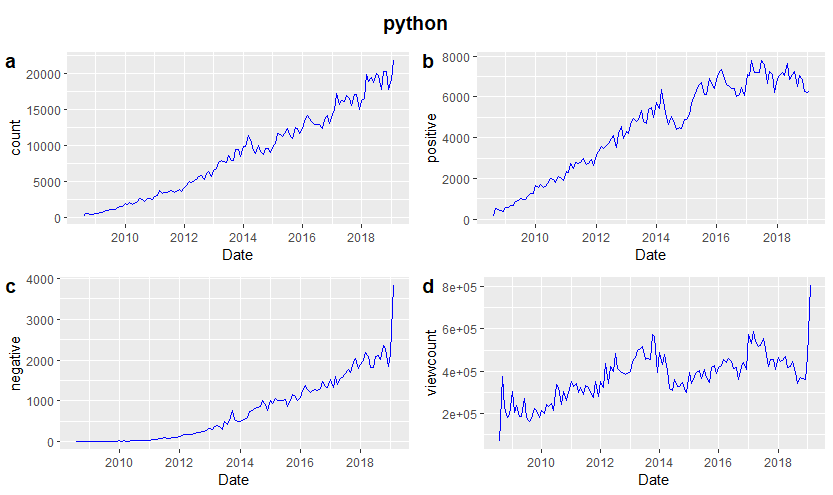
\includegraphics[width=8.5cm]{python.png}
\centering
\caption{Python question count (a), positive count (b), negative count (c), and normalized view count (d)}
\end{figure}


\subsection{RQ1: Language Activity}

\subsubsection{Stack Overflow Annual Surveys}

Table 1 shows the Spearman rho rank correlation coefficients of our SO dataset with the annual SO survey's most popular languages. Each coefficient is on a scale from -1 to +1 and represents the strength of correlation between the ranks of the languages within our Stack Overflow dataset and the languages answered most by surveyed users.

\begin{table}[htbp]
\caption{Stack Overflow Survey and SO Dataset Spearman Correlation}
\begin{center}
\begin{tabular}{|c|c|c|c|c|}
\hline
\textbf{Year} & \textbf{Questions} & \textbf{Positive} & \textbf{Negative} & \textbf{Views} \\
\hline
 2013 & 0.6216 & 0.6121 & 0.7216 & 0.6887 \\
 \hline
 2014 & 0.7748 & 0.7420 & 0.8002 & 0.7958 \\
 \hline
 2015 & 0.7802 & 0.7885 & 0.8258 & 0.7642 \\
 \hline
 2016 & 0.8256 & 0.8011 & 0.8425 & 0.8502 \\
 \hline
 2017 & 0.8460 & 0.8255 & 0.8966 & 0.8123 \\
 \hline
 2018 & 0.8591 & 0.7962 & 0.9268 & 0.8735 \\
 \hline
 2019 & 0.8845 & 0.8256 & 0.9076 & 0.8626 \\
 \hline
\end{tabular}
\label{tab1}
\end{center}
\end{table}

\subsubsection{TIOBE Index}
23 languages on the TIOBE index have their ratings publicly available. Table 2 contains Pearson correlation coefficients between each language's time series within our SO data set and the TIOBE index rating time series.

\begin{table}[htbp]
\caption{TIOBE Index and SO Dataset Pearson Correlation}
\begin{center}
\begin{tabular}{|c|c|c|c|c|}
\hline
\textbf{Language} & \textbf{Questions} & \textbf{Positive} & \textbf{Negative} & \textbf{Views} \\
\hline
 objective-c &  0.8888 &  0.8368 &  0.7500 &  0.7506 \\
 \hline
 r &  0.6627 &  0.6489 &  0.6609 &  0.0916 \\
 \hline
 swift &  0.5291 &  0.2846 &  0.3480 & -0.3025 \\
 \hline
 sas &  0.5169 &  0.1756 &  0.7164 & -0.1477 \\
 \hline
 go &  0.5079 &  0.6460 &  0.2054 &  0.5883 \\
 \hline
 matlab &  0.2995 &  0.0290 &  0.4863 & -0.5471 \\
 \hline
 sql &  0.2782 &  0.3240 &  0.0339 & -0.3748 \\
 \hline
 assembly &  0.2452 & -0.1077 &  0.4772 & -0.2923 \\
 \hline
 vba &  0.1910 &  0.4171 & -0.2512 &  0.3608 \\
 \hline
 python &  0.1617 & -0.0668 &  0.2773 & -0.0783 \\
 \hline
 c\# &  0.1447 &  0.6456 & -0.4242 &  0.7537 \\
 \hline
 groovy &  0.0994 &  0.1783 &  0.1698 &  0.4442 \\
 \hline
 c & -0.0117 &  0.3860 & -0.4495 &  0.6025 \\
 \hline
 dart & -0.0539 & -0.1180 &  0.0750 &  0.5721 \\
 \hline
 javascript & -0.0734 & -0.2563 &  0.1385 & -0.4857 \\
 \hline
 scala & -0.2423 & -0.4811 &  0.4165 & -0.2306 \\
 \hline
 java & -0.3734 & -0.2088 & -0.4084 & -0.1031 \\
 \hline
 perl & -0.4584 & -0.1518 & -0.5749 &  0.3380 \\
 \hline
 vb.net & -0.5803 & -0.7660 &  0.2529 & -0.6393 \\
 \hline
 ruby & -0.5956 & -0.5299 & -0.2662 & -0.3564 \\
 \hline
 c++ & -0.6175 & -0.2536 & -0.8373 &  0.4132 \\
 \hline
 delphi & -0.7018 & -0.4713 & -0.3734 & -0.5075 \\
 \hline
 php & -0.7965 & -0.5534 & -0.8910 & -0.1058 \\
 \hline
\end{tabular}
\label{tab1}
\end{center}
\end{table}

\subsubsection{Employability}
Many duplicate jobs are posted across the large job search sites considered, so we take the average of the counts for language related jobs instead of the total for a fairer ranking of languages. Figure 3 shows a time series of the Spearman rank correlation coefficients between the ranking of languages each month in the SO dataset and current job postings today.

\begin{figure}[h]
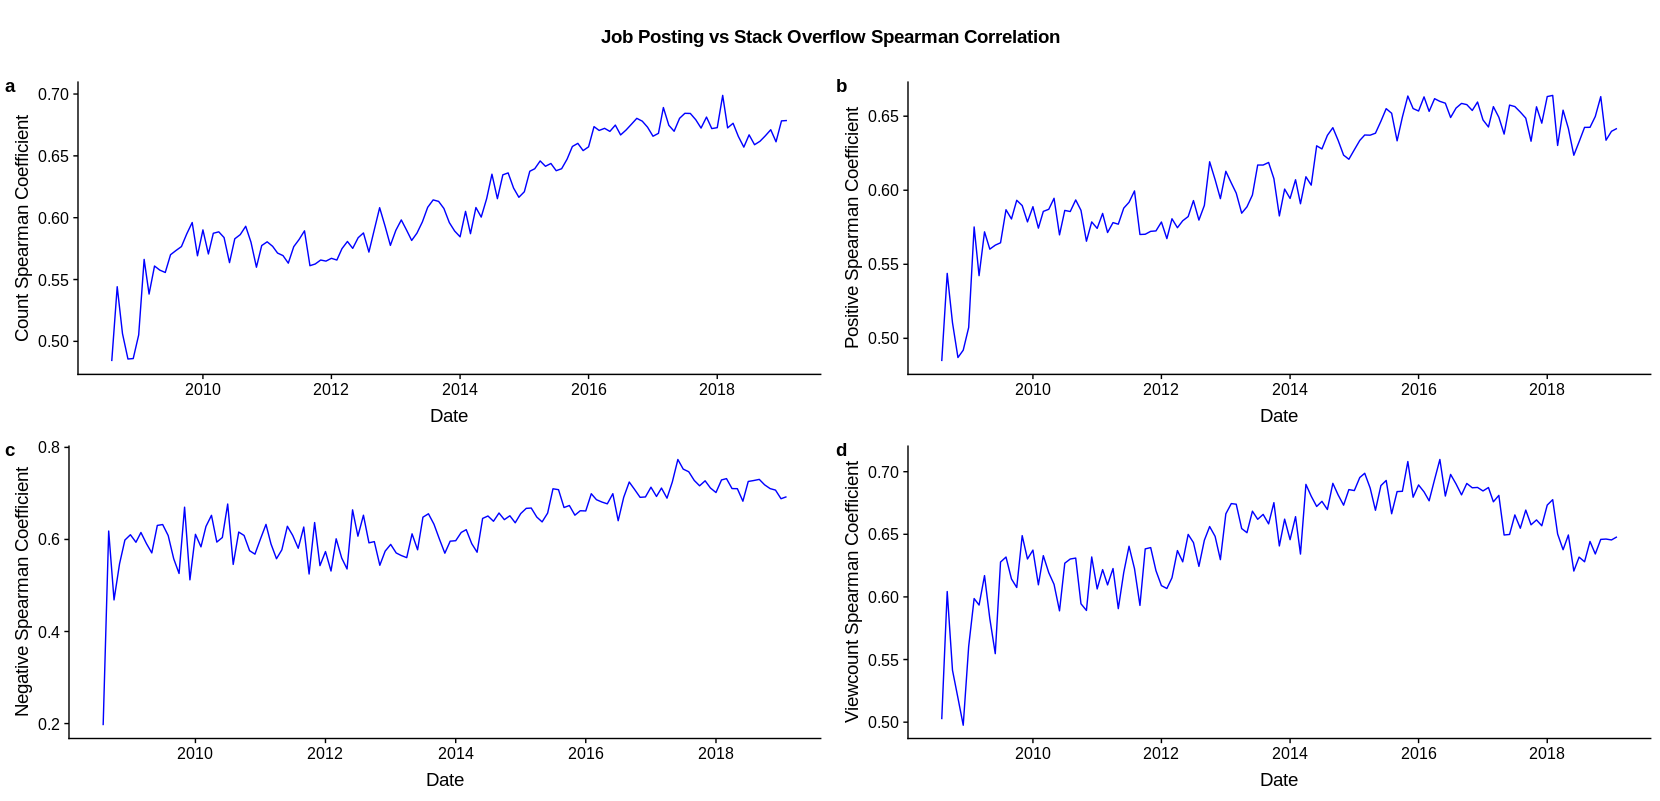
\includegraphics[width=8.5cm]{Jobspearman.png}
\centering
\caption{Spearman rank correlations between job postings in June 2019 and SO questions (a), positive questions (b), negative questions (c), and question viewcounts (d)}
\end{figure}

\subsection{RQ2: Language Categorizing and Relations}

\subsubsection{Time Series Clustering}
Figure 4 shows the shape-based distance hierarchical clustering done on the time series of each language's question count. The height of each node is proportional to the value of the inter-group dissimilarity between its two daughter nodes. Clustered nodes show the most similar time series shapes as their sister nodes. The same clustering is done for the other 3 metrics.

\begin{figure*}[h]
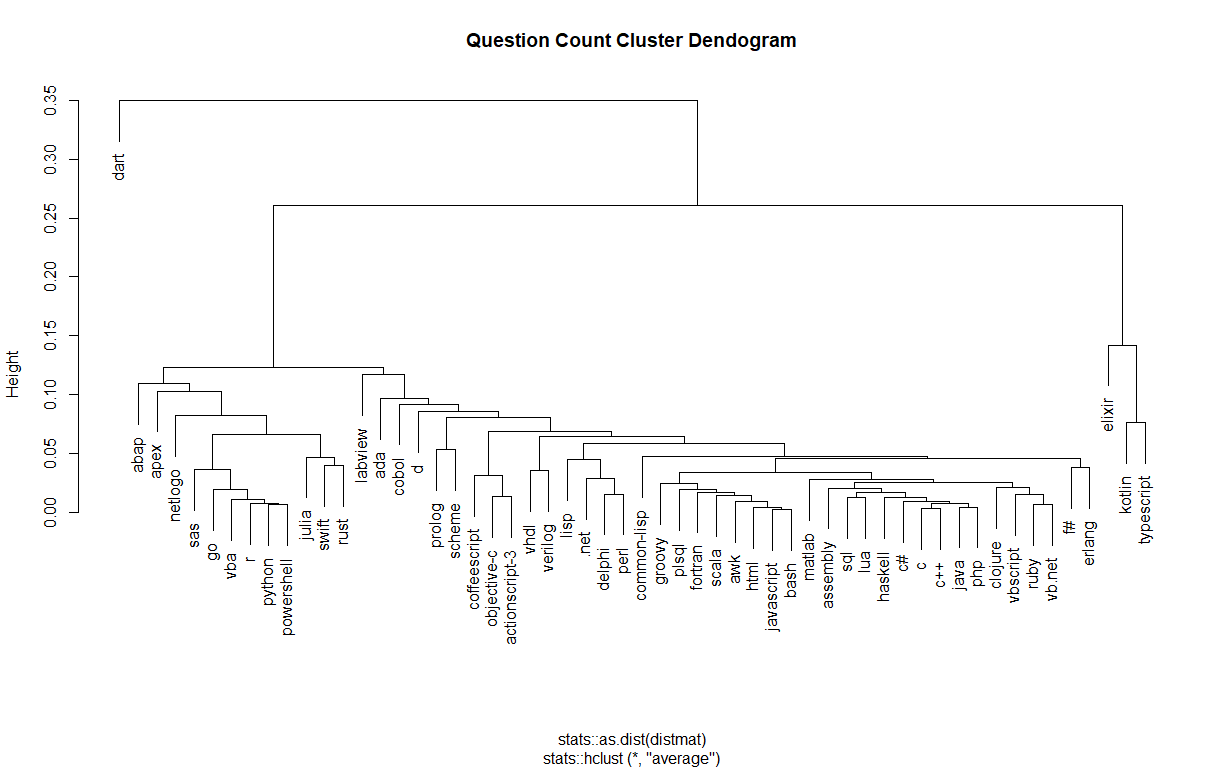
\includegraphics[width=16cm]{countclust.png}
\centering
\caption{Shaped-Based Distance Hierarchical Clustering of Language Question Counts}
\end{figure*}

\subsubsection{Linear Dependence Relations}

Each language's four metric time series are correlated with each other language's time series. Each language produces a table of Pearson linear dependence correlation coefficients. A high positive coefficient implies languages with similar time series shapes, where the two languages positively affect eachother. On the contrary, high negative correlations imply opposite shapes, where languages negatively affect eachother. Positive correlations are expected to match the clustering algorithm above, while negative correlations are not depicted in the clustering. Table 3 is an example of the correlations between R and the top 10 question count coefficients.

\begin{table}[htbp]
\caption{R Top 10 Question Count Pearson Correlations}
\begin{center}
\begin{tabular}{|c|c|c|c|c|}
\hline
\textbf{Language} & \textbf{Questions} & \textbf{Positive} & \textbf{Negative} & \textbf{Views} \\
\hline
python &  0.9864 &  0.9752 & 0.9518 &  0.7937 \\
\hline
powershell &  0.9862 &  0.9411 & 0.9277 &  0.7570 \\
\hline
vba &  0.9774 &  0.9545 & 0.9551 &  0.7541 \\
\hline
go &  0.9760 &  0.9411 & 0.8053 &  0.7806 \\
\hline
scala &  0.9332 &  0.8562 & 0.9132 &  0.7212 \\
\hline
julia &  0.9279 &  0.8602 & 0.6476 &  0.4798 \\
\hline
rust &  0.9154 &  0.8592 & 0.6830 &  0.5274 \\
\hline
sas &  0.9107 &  0.8270 & 0.8500 &  0.7313 \\
\hline
javascript &  0.9009 &  0.8704 & 0.9452 &  0.7439 \\
\hline
bash &  0.8922 &  0.7997 & 0.9397 &  0.1348 \\
\hline
\end{tabular}
\label{tab1}
\end{center}
\end{table}

\section{Discussion}

\subsection{RQ1: Language Activity}

\subsubsection{Stack Overflow Surveys}
The rho coefficients show that each of the five metrics form a strong correlation with the survey results. This increases the plausibility that the four metrics can be used to gauge a programming language's popularity overall. What survey respondents believe to be popular languages is reflected in the amount of questions asked and views on said post in our dataset. The correlations hover between 80\%-90\% in recent years, and we consider this an aforementioned strong correlation because tens of thousands of survey responders are representing the millions of SO users, we can not expect a near 100\% correlation.

We observe that the correlation becomes stronger in more recent years. This is very likely due to the amount of users participating in the survey greatly increasing in the later years, thus the survey would greater reflect the Stack Overflow community as a whole (10,000 users in 2013, over 100,000 in 2018). We also observe that on average, the amount of negatively rated questions best correlates with the survey results. Perhaps this means that the amount of poor and irrelevant questions being asked best represents the amount of activity within a language.

We believe our four metric dataset is a good representation of the activity and popularity of a language within Stack Overflow.

\subsubsection{TIOBE Index}

We observe that there are few languages with more than a weak correlation with the TIOBE index. Few languages have a strong correlation (+0.80), and the majority have very weak correlations (or negative). The mean Pearson correlation coefficients for total question count, positive count, negative count, and viewcount are respectively: 0.0009, 0.0264, 0.0231, and 0.0323.

The averages are very weak correlations, the only languages that showed high correlations were languages with very sharp increases or decreases in activity during the timeline of both datasets (after 2008). The correlations are inconsistent, so overall, we conclude that our SO dataset does not show a relation with TIOBE's search engine dataset.

We believe that while TIOBE's dataset does show the accurate popularity of a language, its possible that our dataset better shows the current activity of programming language users. Our dataset may also better predict the future popularity of a language which would skew our correlation values, but that is not covered in this study.

\subsubsection{Employability}

Figure 3 shows that in general, the SO dataset has a relatively strong correlation with current job postings. We observe that negatively received question counts provide (once again) the highest rank correlation; specifically the ranks from a few months prior produce the highest coefficients. 

The correlation is not weak, but not extremely strong either. It is likely that the majority of questions being asked on SO come from users also currently employed (including students) and not those looking for employees. Although, if current questions do not best represent current openings, perhaps they represent future openings.

We cannot draw a conclusion from this result because we only have access to current postings. Job search websites (that we know of) do not archive past posts, so it is only possible to compare with current posts. We cannot determine if the strong correlation we obtained is a coincidence or not.

\subsection{RQ2: Language Categorizing}

Table 3 shows the top 10 question count correlations with R. Note that the languages most correlated with R in the question section were also clustered near R in Figure 4. This increases the validity of using Pearson linear dependence correlation to find languages with similar trends.

Figure 5 shows R question counts next to Python, Go, and VBA. We smooth the graphs for visual aid. The smoothing was done using a moving average best fit curve with a span of 0.1 (using geom\_smooth in the R package ggplot2). 

\begin{figure*}[h]
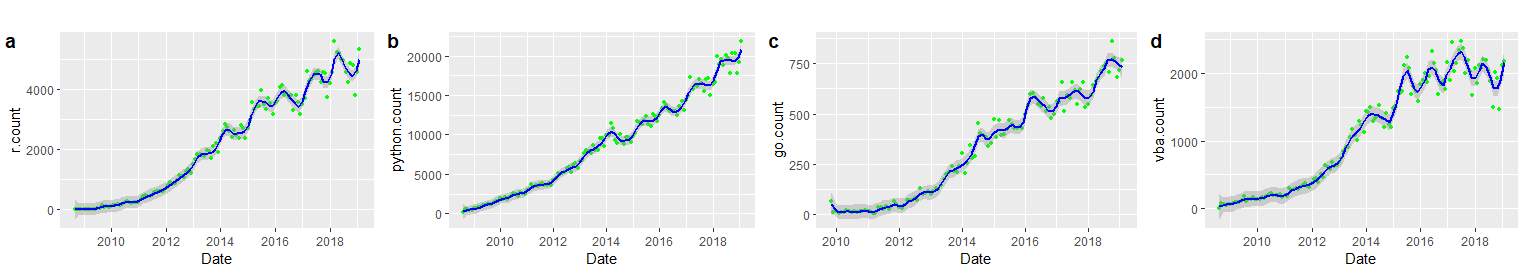
\includegraphics[width=16cm]{Rtop4.png}
\centering
\caption{R Top Question Count Correlations: Python (b), Go (c), and VBA (d)}
\end{figure*}

First to note in Figure 5 is that the shapes are very similar on a relevant scale (not absolute), but the trend of always increasing is the same. All languages show very similar shapes and near identical trends with languages they have a correlation coefficient higher than +0.9 with.

A more interesting example is Figure 6 which shows the top 4 question count correlations with Assembly which are: C, Java, Haskell, and C++. Note that the number of questions experience a sharp rise in September, a small fall in December, a small rise in January, and a sharp fall during May. This trend exactly follows the USA school year. Because these languages show this trend, we can categorize the 5 languages as having a primary use of being taught in school.

\begin{figure*}[h]
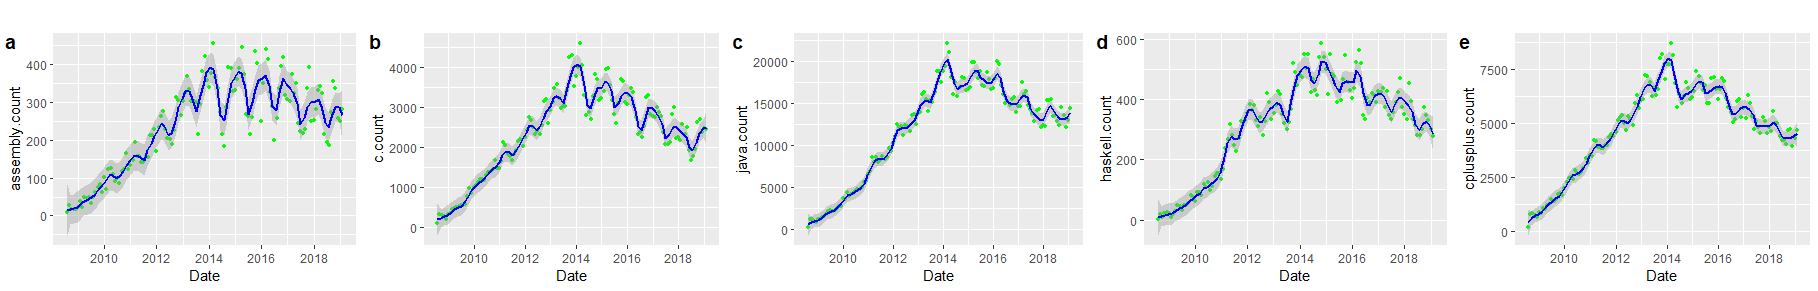
\includegraphics[width=16cm]{schoolgroup.png}
\centering
\caption{Assembly Top Question Count Correlations: C (b), Java (c), Haskell (d), and C++ (e)}
\end{figure*}

\vspace{5mm}

Pearson correlation also provide negative values, which would signify a negative relationship between languages. We expect that highly negatively correlated languages experience rises and falls at opposite times, and that the languages have negative impacts on one another. Figure 7 gives two examples: Swift and Objective-C having a negative relationship, and Rust and .net having a negative relationship. Also note that negative relationships cannot be found through our first method of shape-distance based clustering.

\begin{figure}[h]
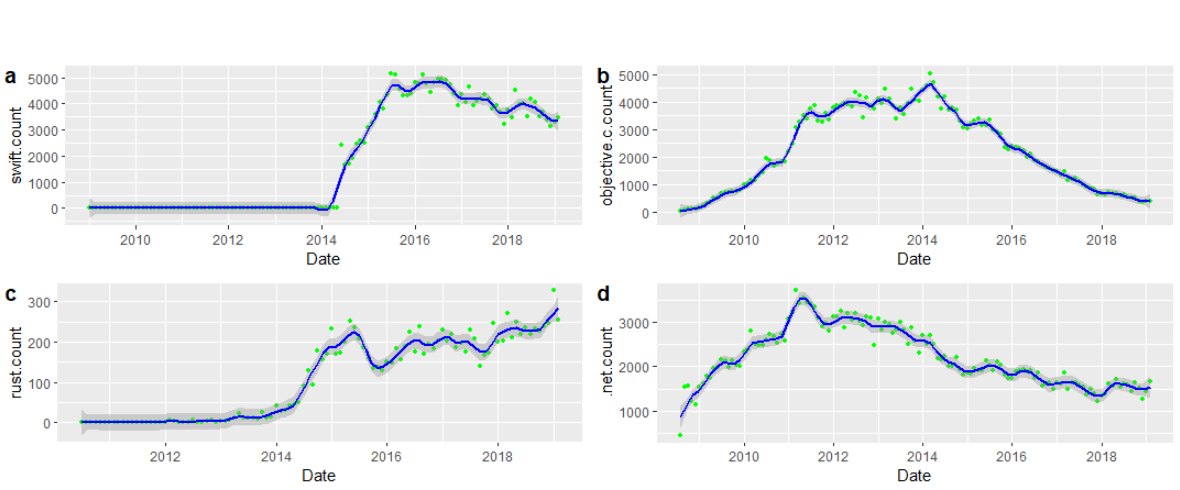
\includegraphics[width=8.5cm]{counters.png}
\centering
\caption{Question counts of Swift (a) vs Objective-C (b) and Rust (c) vs .net (d)}
\end{figure}

There are many more examples of relations to be found between languages. However, for the sake of brevity, we only show three examples in this paper.

We can conclude from even the few relations we have provided that relations between programming languages, frameworks, and also topics in general can be found quite easily by looking at the Stack Overflow dataset. Perhaps in the future, such relations can be used to predict which programming languages will grow in activity as well as which should be adopted for certain environments or programs.

\section{Related Works}

Anton Barua, Stephen W. Thomas, and Ahmed E. Hassan do an analysis on topics and trends within Stack Overflow \cite{SOtalking}, and their impact value produces a similar result with our Pearson correlation coefficients. Our study is a more comprehensive exploration of specifically programming languages and not only trends, but the relationships between languages as well, which builds on some of the results they share.

Christoph Treude, Ohad Barzilay, and Margaret-Anne Storey examine how programmers ask questions on the web \cite{progquestions}, and specifically what type of questions programmers tend to ask on Q\&A websites such as Stack Overflow.

David Smith, and Azad Ali analyze job postings on Dice.com to find which languages were the most employable over time \cite{jobanalyze}. 

\vspace{5mm}


\section{Threats to Validity}

In RQ1, we needed to determine a metric for which programming languages to consider when retrieving the tagged questions from the Stack Overflow dataset. According to Wikipedia, thousands of programming languages exist, but the vast majority are used by very few people. Thus, we decided to consider the current top 100 languages listed on the TIOBE index. We believe the 100 languages listed there to be the best representation of significant programming languages within the online community.

However, by reducing the number to 100, we may have differed our rank correlation results slightly for the Stack Overflow surveys and job search websites in opposition to if we considered all existing programming languages. The TIOBE linear dependence correlation is not affected by this problem. Also, if certain languages were very popular years ago, but are not in the top 100 today, they were not considered for this study which may have affected our results further.

TIOBE has not released their method of calculating their ratings and rankings, so there are questions of its validity. However, the index is well-cited, and we believe that every significant programming language was considered. Therefore, this threat is insignificant.

\bibliographystyle{./bibliography/IEEEtran}
\bibliography{./bibliography/IEEEabrv}


\end{document}
